\chapter{Results}

This chapter presents the outcomes of testing the developed mobile application for real-time museum exhibit recognition. The evaluation was conducted directly at the Museum of Decorative Arts in Prague (\textit{Uměleckoprůmyslové museum v Praze} or UPM), where the videos for our training dataset were recorded. UPM gathers, curates, and preserves historical and contemporary collections of applied arts, design, and artistic craftsmanship for future generations. The main goal for this testing was to verify whether the performance achieved in the initial validation phase (Chapter~\ref{chapter:model_training}) corresponds with real-world application scenarios within the museum environment.

\section{Testing Procedure}

The guidelines were established before testing to maintain consistency and repeatability. Each test was performed by pointing the smartphone camera at selected museum exhibits from different but reasonable angles, trying to replicate typical user scenarios. The testing was conducted twice: in the morning and in the evening, allowing us to measure the model's robustness under different lighting conditions (which, however, were not much different due to the museum's indoor lighting). The application was run on a Samsung Galaxy S9 smartphone.

Due to changes in UPM's exhibition collections between the creation of the dataset and the time of testing, not all exhibits initially present in our dataset were still accessible. Therefore, for practical evaluation purposes, we found a subset of 80 available exhibits covering a diverse range of kinds and sizes, including furniture, sculptures, paintings, clothes, toys, jewelry, and glass art.

\section{Classification Results and Accuracy}

The results were the same for both morning and evening testing. Out of the 80 exhibits chosen for the evaluation, the application correctly identified 75 of them at the first attempt, which equals an accuracy rate of approximately 93.75\%. Importantly, the five misclassified exhibits were nevertheless found among the alternative predictions displayed to the user.

Three of the five misclassifications were sculptures, which were visually similar to one another, and the remaining two were a glass artwork and a painting, which again had very similar counterparts in the training dataset. The model was the most confident about toys and furniture, since there was much more diversity between them: they were of different shapes, colors, and sizes, while the sculptures were more challenging due to their similar forms and materials.

This result aligns closely with our validation set results obtained during the training phase (where validation accuracy was around 95.9\% after fine-tuning). Observing that real-world accuracy was only slightly lower is encouraging, as this confirms that the model is generalizing appropriately.

\section{Inference Time and Responsiveness}

A critical aspect of our testing was checking the application's real-time responsiveness, as slow predictions would negatively affect user experience. Thanks to the implemented Debug Mode, inference time measurements (the time required for the model to produce predictions from input images) could be observed and recorded directly within the mobile application during testing.

On average, inference times remained stable at around 120--150 ms. This performance is beneficial for seamless and smooth recognition, especially important when visitors move with their devices through exhibitions. Such fast classification guarantees minimal latency observable to the human eye, providing an actual real-time experience. Additionally, the achieved inference time would not have been possible with alternative methods such as the embedding-based similarity search approach, which typically requires more extensive search space computations. Thus, our chosen method, direct classification via MobileNetV2 and TensorFlow Lite integration, was confirmed to be the most suitable for practical museum deployments on mobile devices.

\section{Confidence Levels and Threshold Evaluation}

During the real-world testing sessions, we also monitored prediction confidence levels generated by the model to assess our chosen classification threshold value (0.3). For most correctly identified exhibits, the confidence scores ranged between 0.5 and 1.0. Typically, larger and visually distinguishable items were consistently predicted with confidence values above 0.8, whereas smaller or visually less distinctive exhibits fell towards lower confidence scores, around 0.5--0.7.

Nevertheless, despite observing relatively higher confidence values for correctly classified items, we maintained the lower threshold of 0.3 initially chosen during development. This was done to ensure that the correct exhibit could still be found among the alternatives even in cases of misclassifications.

\section{Visual Results and Demonstration}

To visually document and illustrate real-world app performance and functioning, several photos and a video were recorded during the evaluation process. In Figure~\ref{fig:test_examples}, you can see some examples of the application recognizing various exhibits in the museum.

\begin{figure}[h]
    \centering

    \begin{subfigure}[b]{0.4\textwidth}
        \centering
        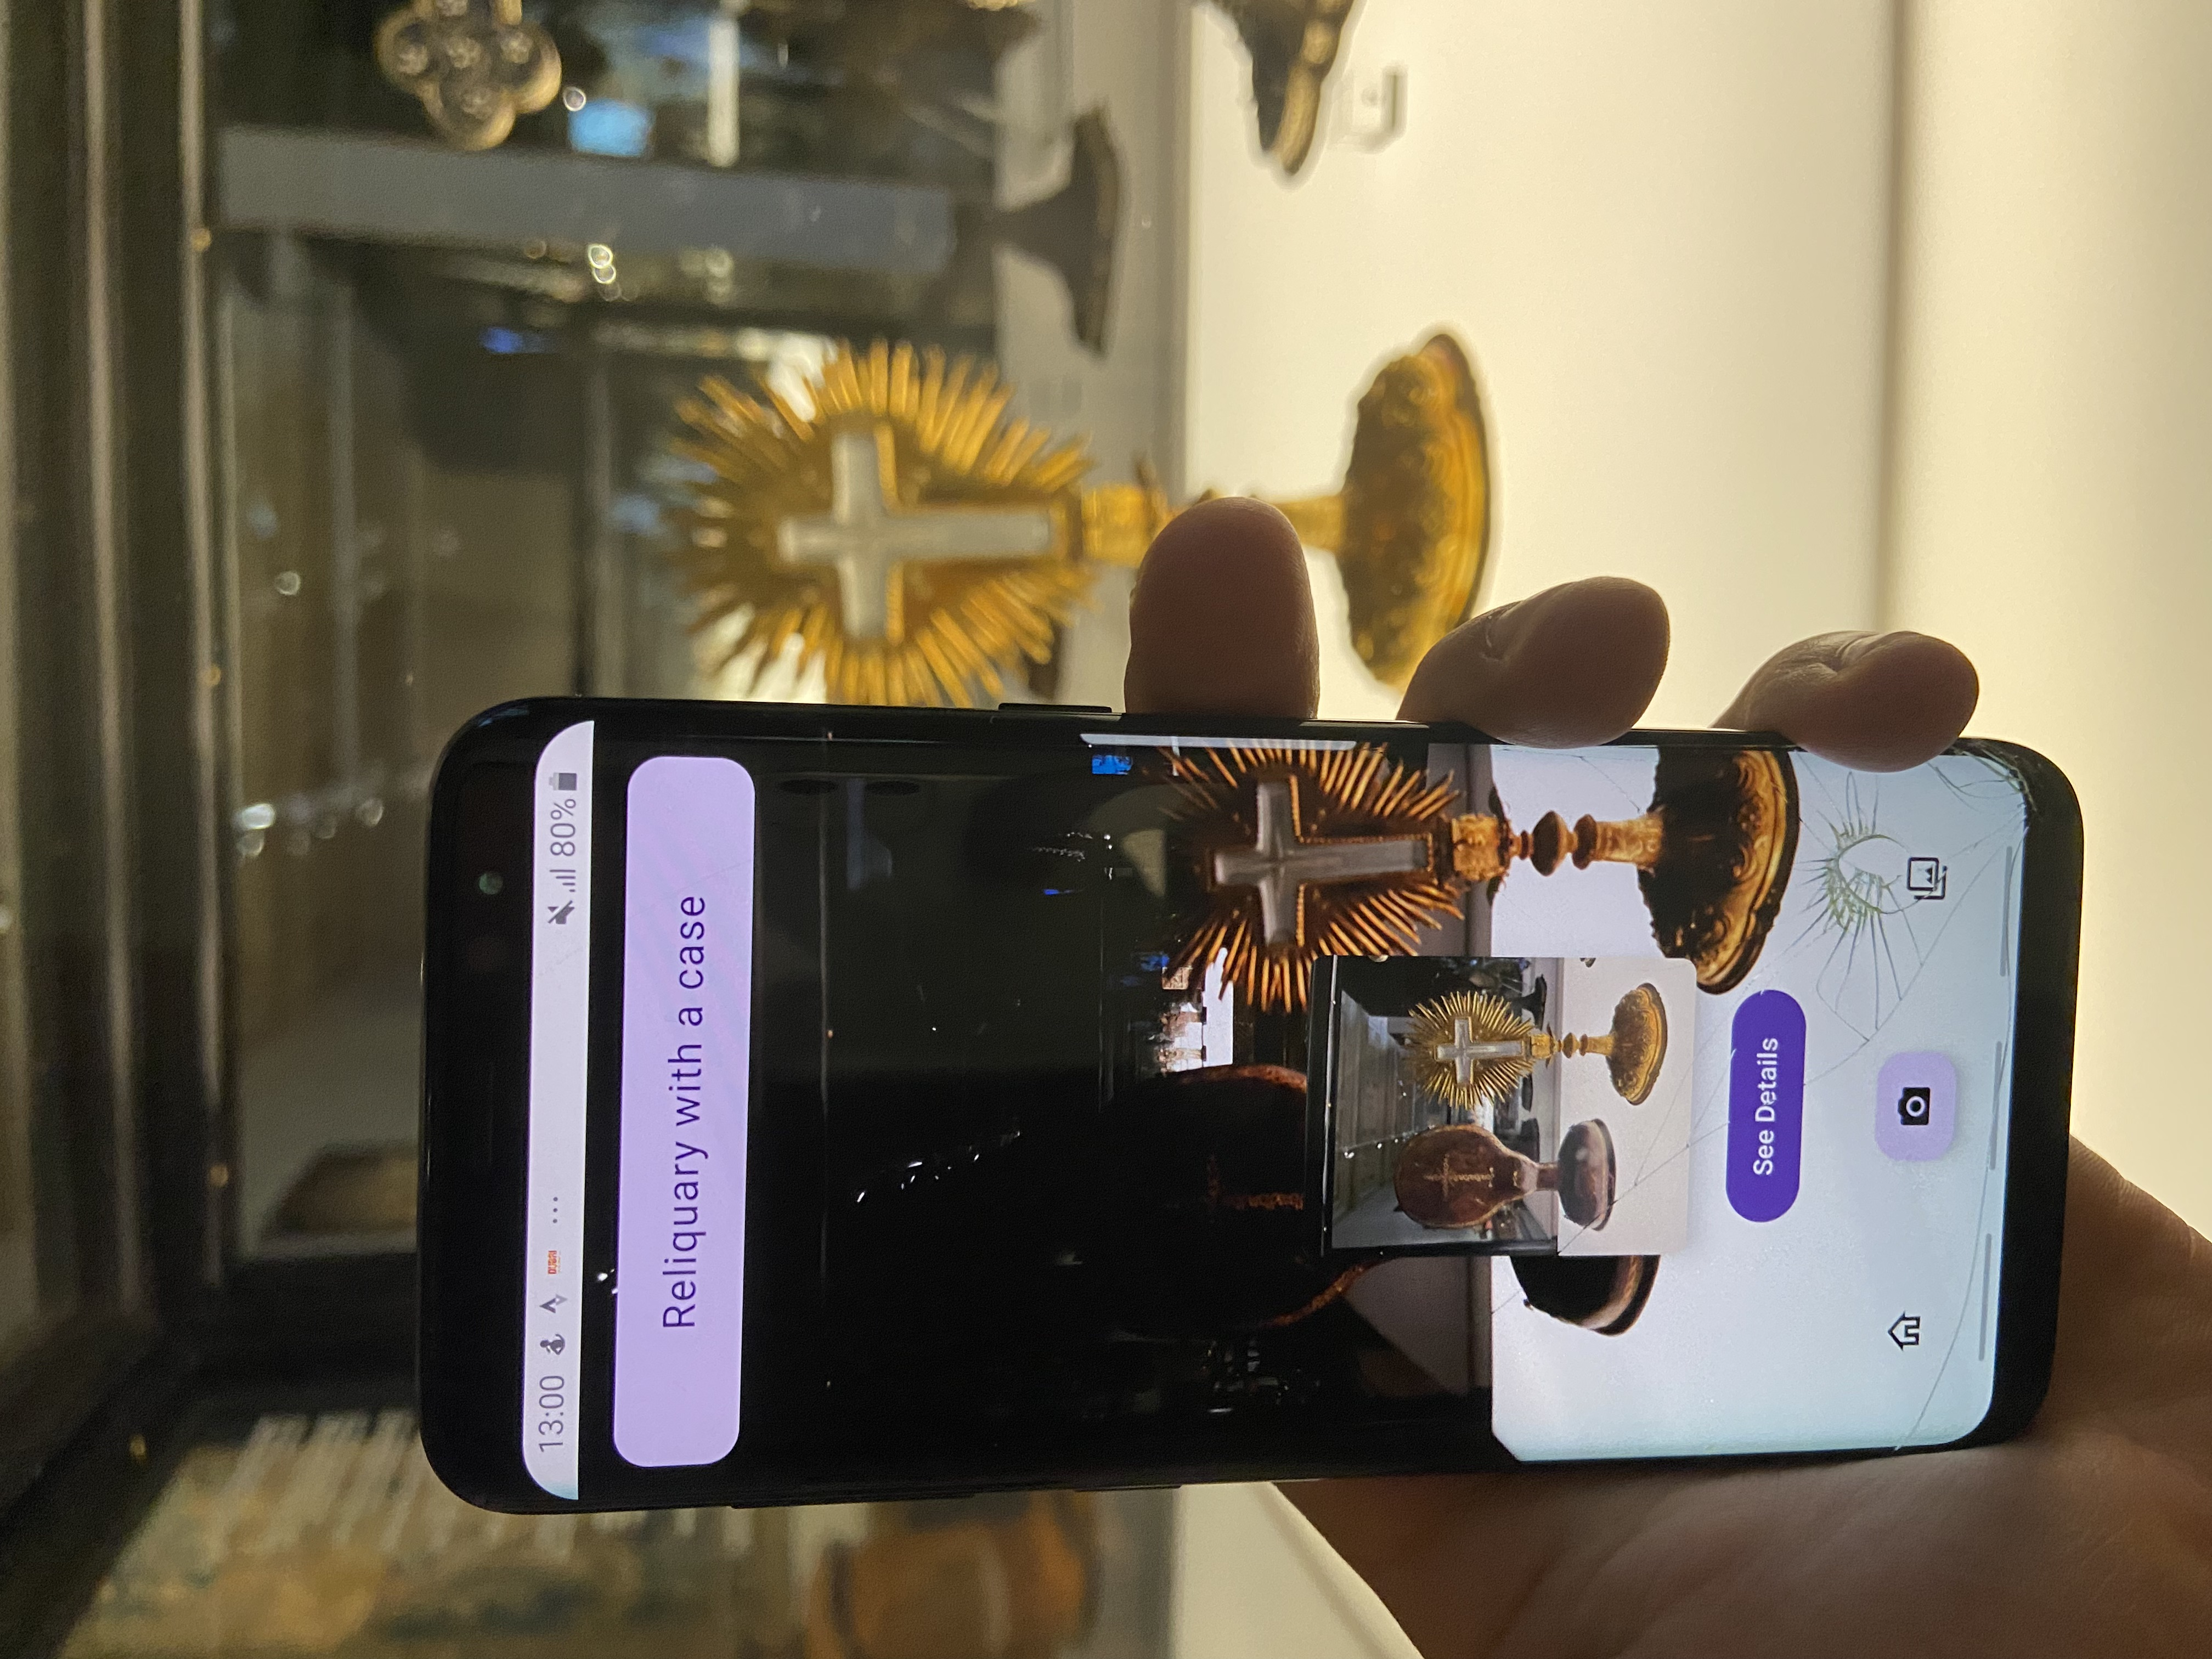
\includegraphics[angle=270, width=\textwidth]{img/test-example-1.jpg}
    \end{subfigure}
    \hfill
    \begin{subfigure}[b]{0.4\textwidth}
        \centering
        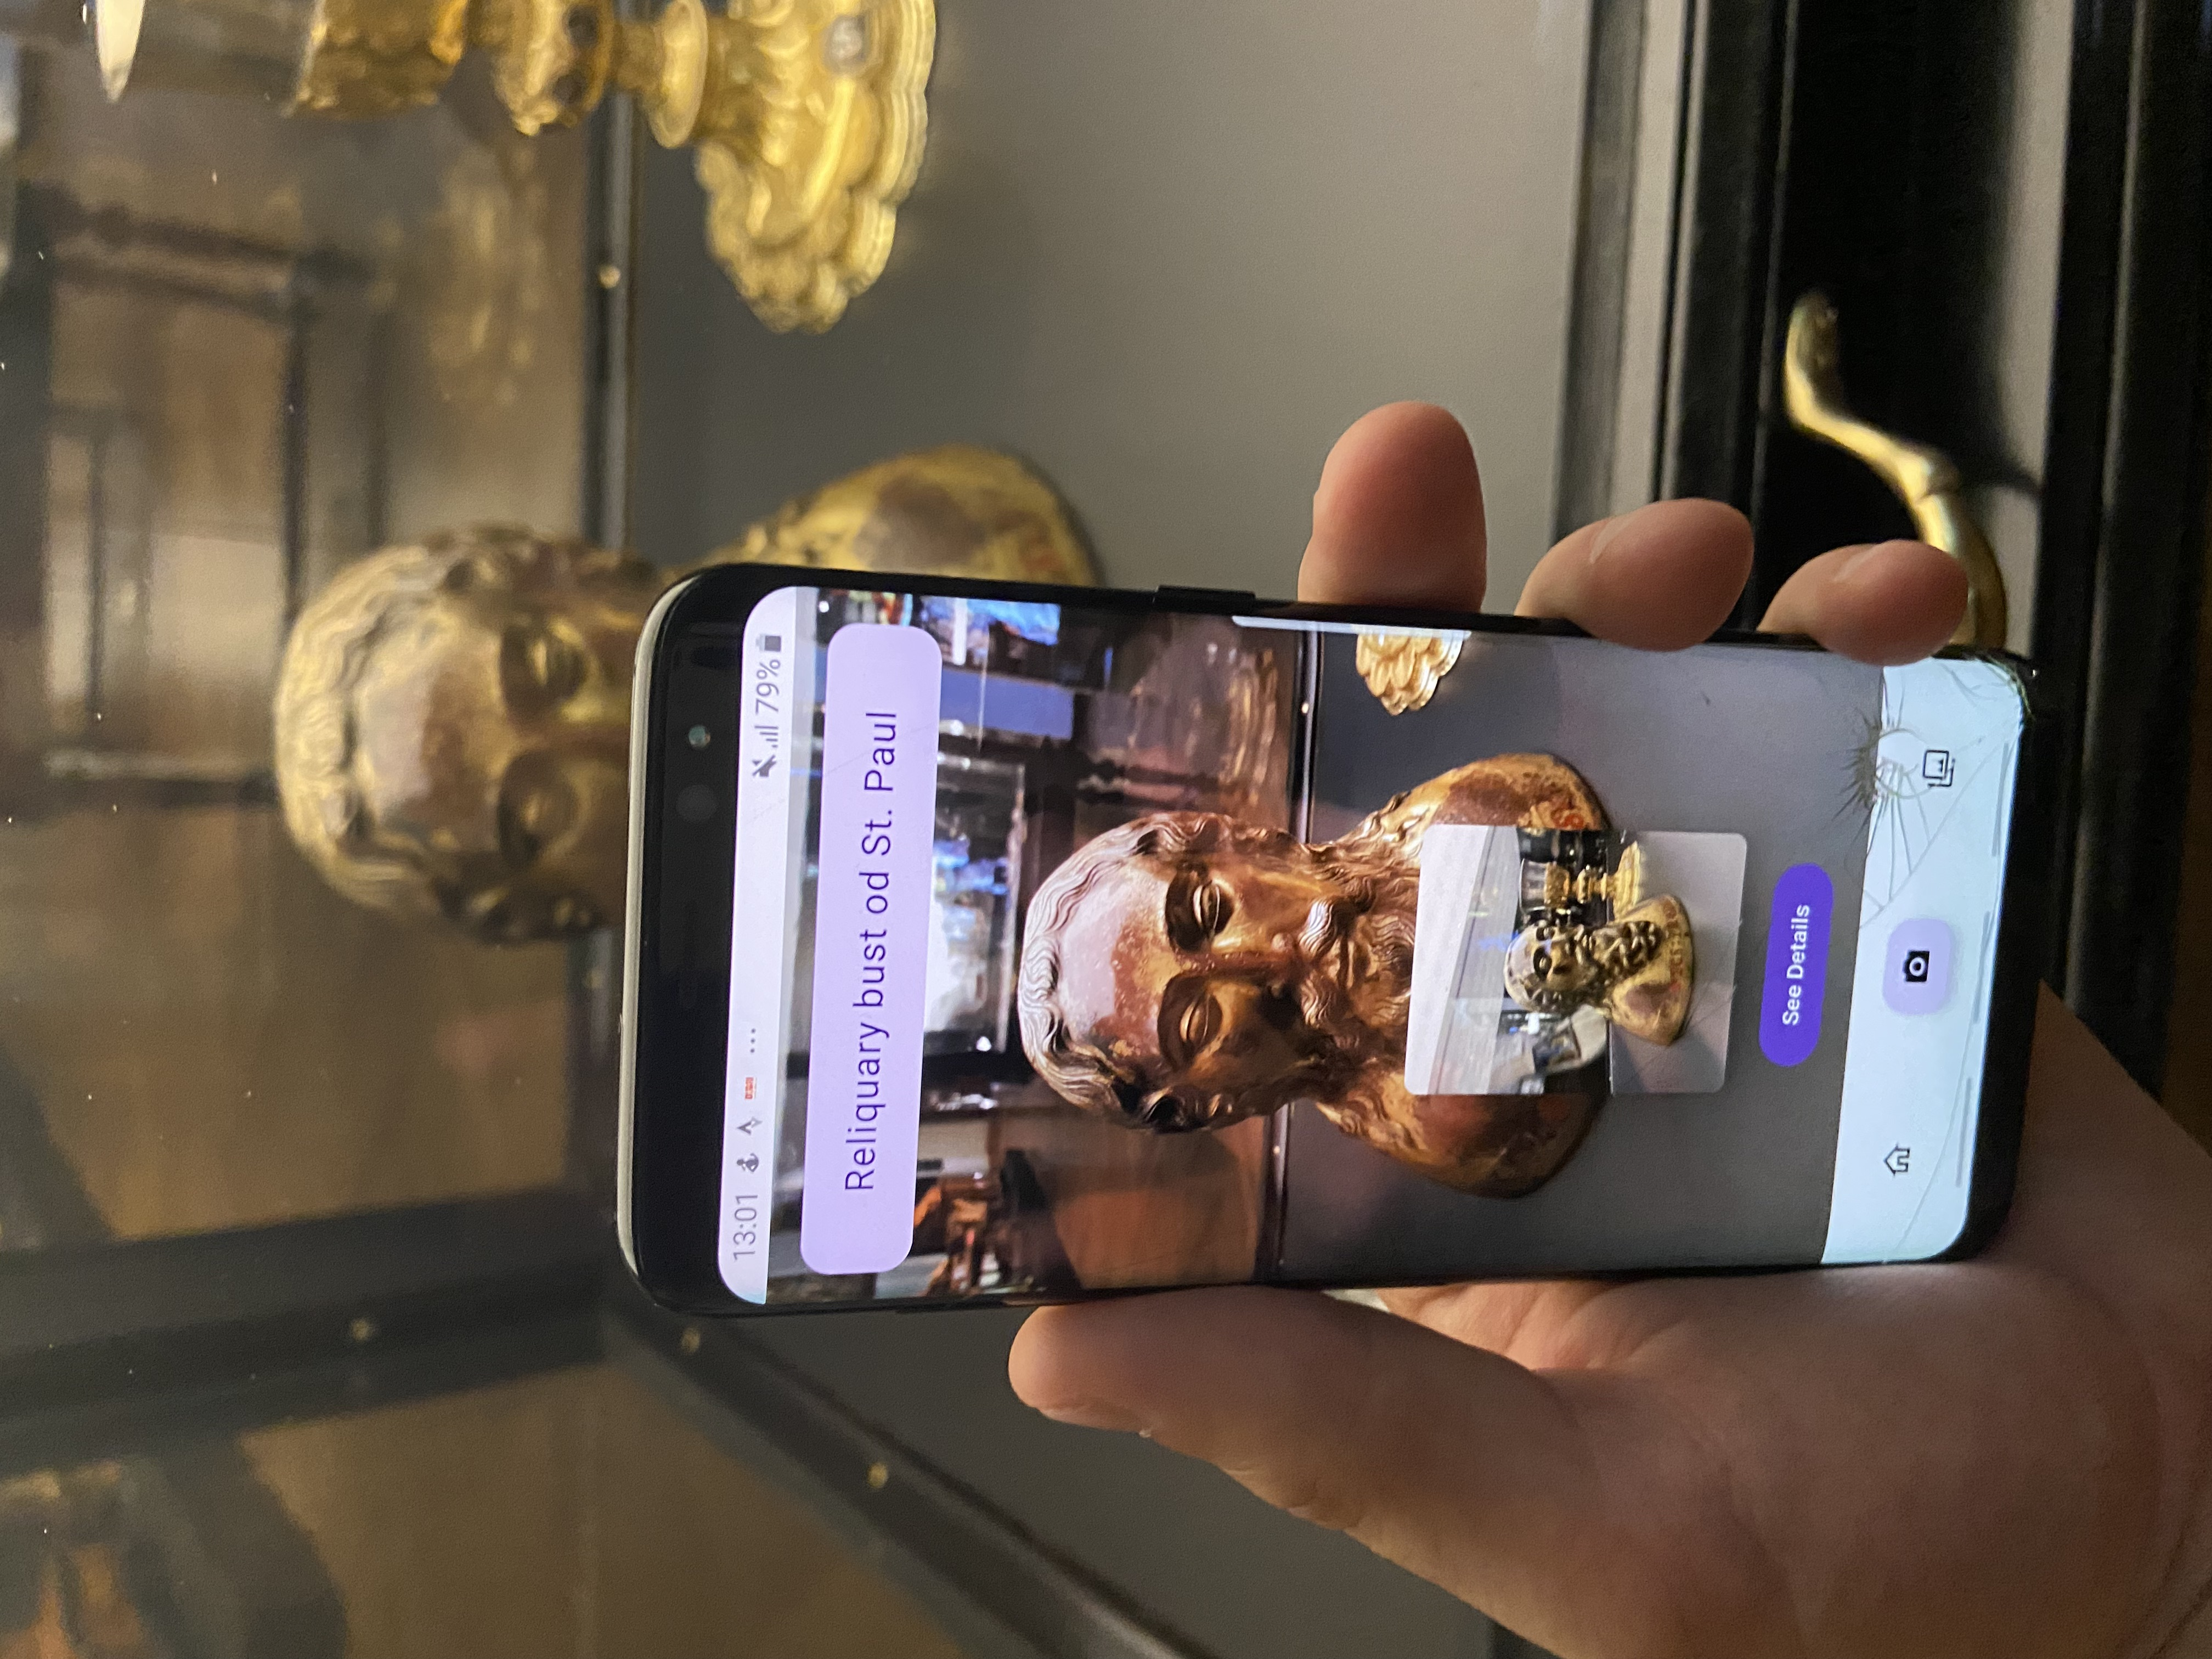
\includegraphics[angle=270, width=\textwidth]{img/test-example-2.jpg}
    \end{subfigure}

    \vspace{1em}

    \begin{subfigure}[b]{0.4\textwidth}
        \centering
        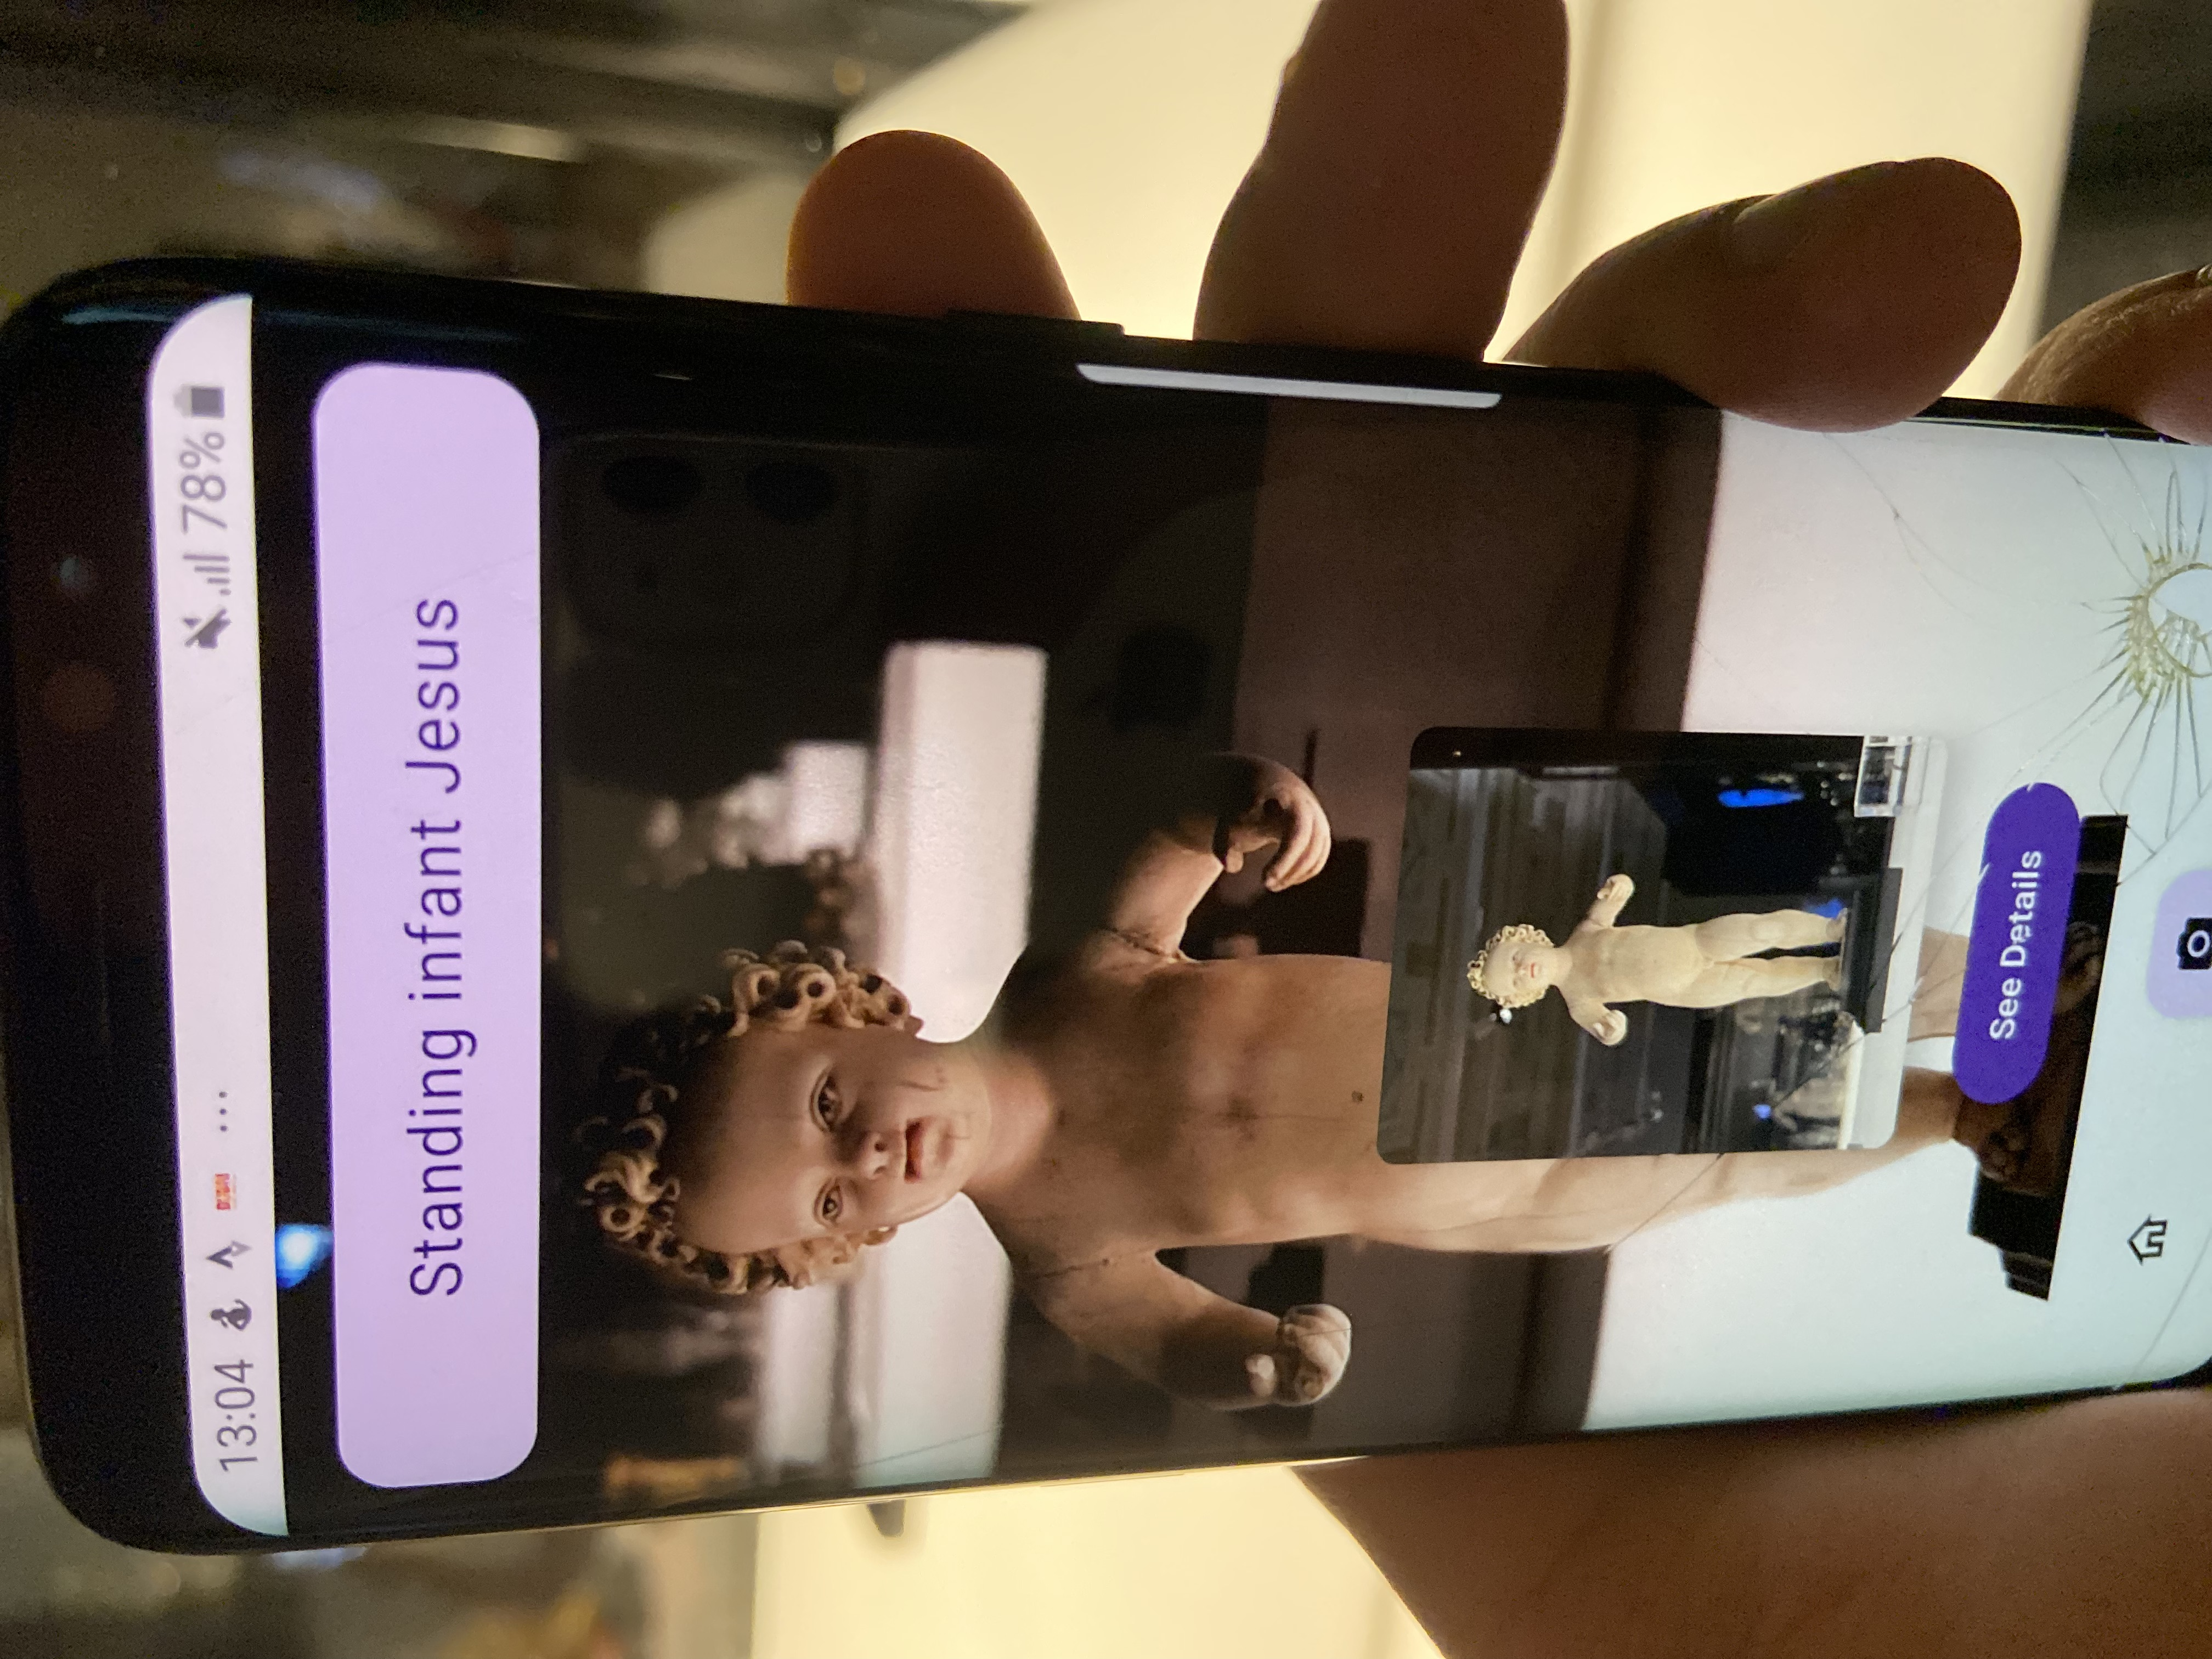
\includegraphics[angle=270, width=\textwidth]{img/test-example-3.jpg}
    \end{subfigure}
    \hfill
    \begin{subfigure}[b]{0.4\textwidth}
        \centering
        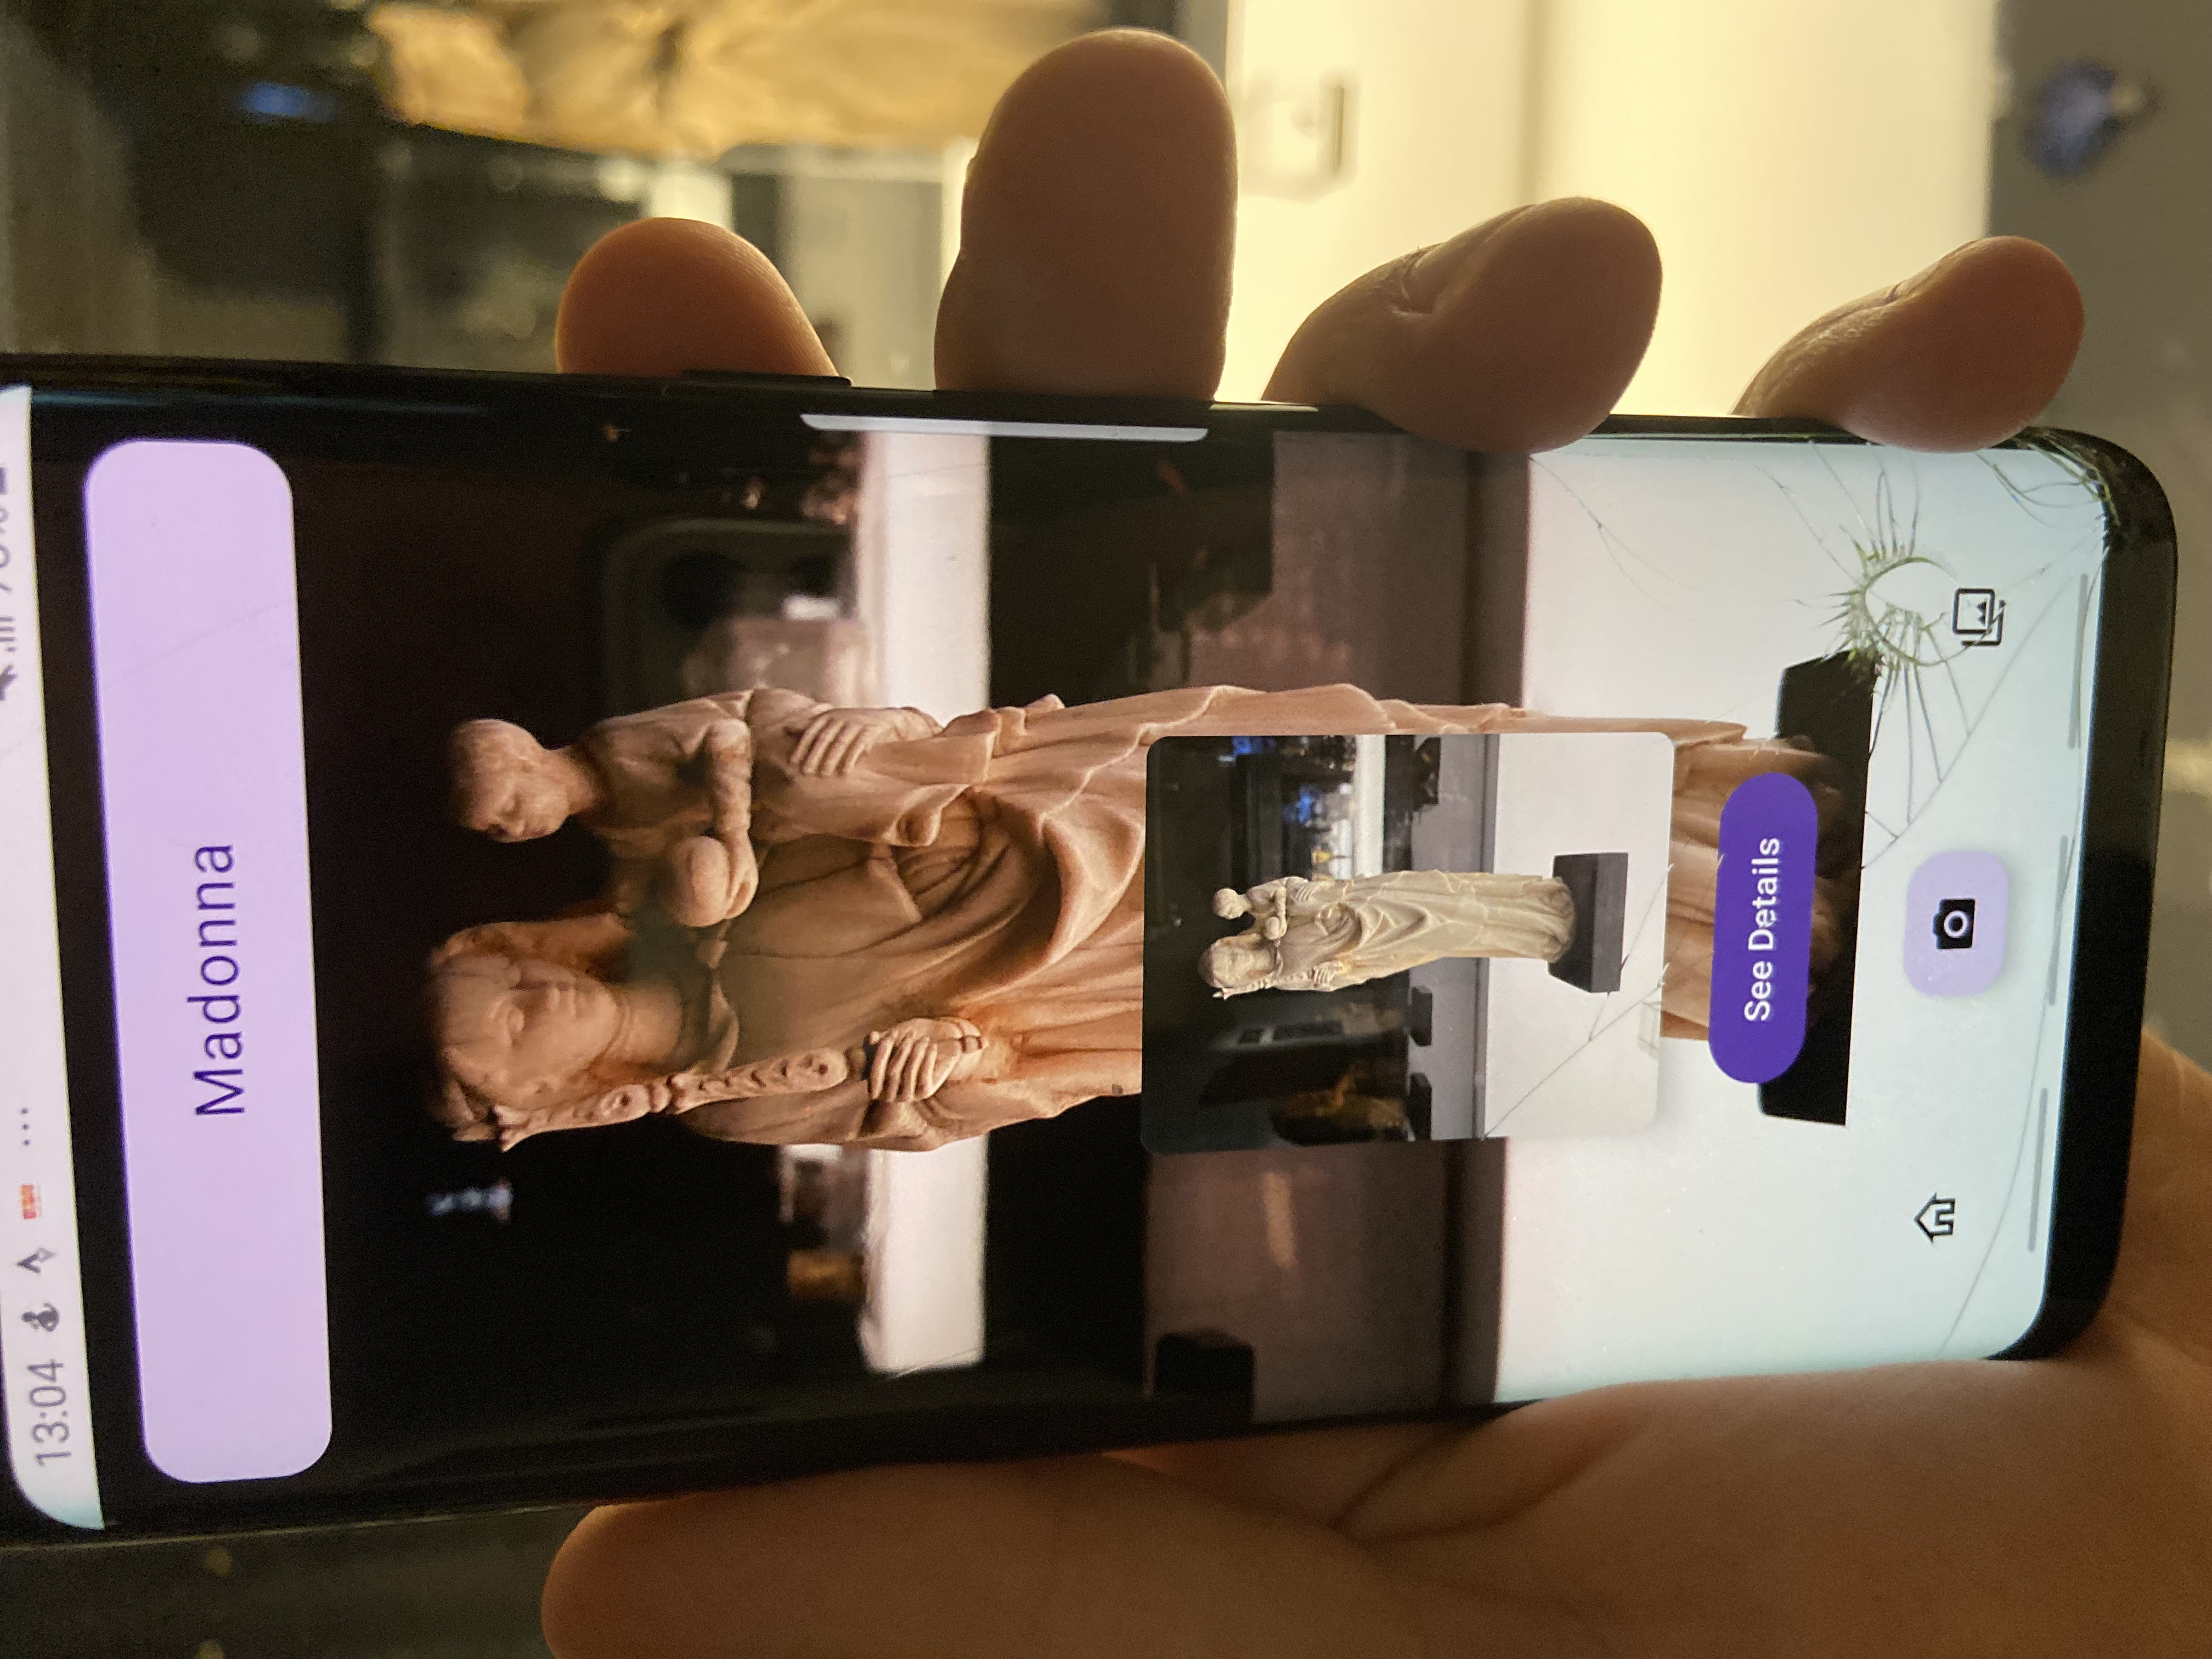
\includegraphics[angle=270, width=\textwidth]{img/test-example-4.jpg}
    \end{subfigure}

    \caption{Examples of real-world exhibit recognition.}\label{fig:test_examples}
\end{figure}

Additionally, a short video demonstrating the application during testing is available here:

\begin{center}
\url{https://www.youtube.com/shorts/eHmp9kK2hn8}
\end{center}

\section{Summary}

In summary, the developed mobile application demonstrated strong performance in real-world museum exhibit recognition, achieving a decent accuracy rate of 93.75\% on a diverse set of 80 exhibits. The application successfully identified most exhibits at the first attempt, with misclassifications being limited to visually similar items, which is a common challenge in image classification tasks. The inference time remained low, ensuring a responsive user experience, and the confidence levels of predictions were consistent with expectations. Overall, the application proved to be a valuable tool for enhancing the museum experience by providing real-time information about exhibits, confirming its practical applicability in real-world scenarios.